%%
%% This is file `sample-sigconf.tex',
%% generated with the docstrip utility.
%%
%% The original source files were:
%%
%% samples.dtx  (with options: `sigconf')
%% 
%% IMPORTANT NOTICE:
%% 
%% For the copyright see the source file.
%% 
%% Any modified versions of this file must be renamed
%% with new filenames distinct from sample-sigconf.tex.
%% 
%% For distribution of the original source see the terms
%% for copying and modification in the file samples.dtx.
%% 
%% This generated file may be distributed as long as the
%% original source files, as listed above, are part of the
%% same distribution. (The sources need not necessarily be
%% in the same archive or directory.)
%%
%%%% Proceedings format for most of ACM conferences (with the exceptions listed below) and all ICPS volumes.
\documentclass[sigconf,nonacm,11pt]{acmart}
%%%% As of March 2017, [siggraph] is no longer used. Please use sigconf (above) for SIGGRAPH conferences.

%%%% Proceedings format for SIGPLAN conferences 
% \documentclass[sigplan, anonymous, review]{acmart}

%%%% Proceedings format for SIGCHI conferences
% \documentclass[sigchi, review]{acmart}

%%%% To use the SIGCHI extended abstract template, please visit
% https://www.overleaf.com/read/

% [ packages ] --------------------------------------------

% [ /packages ] -------------------------------------------

%%
%% \BibTeX command to typeset BibTeX logo in the docs
\AtBeginDocument{%
  \providecommand\BibTeX{{%
    \normalfont B\kern-0.5em{\scshape i\kern-0.25em b}\kern-0.8em\TeX}}}

\graphicspath{{fig/}{./}}

%%TC:ignore
%% Rights management information.  This information is sent to you
%% when you complete the rights form.  These commands have SAMPLE
%% values in them; it is your responsibility as an author to replace
%% the commands and values with those provided to you when you
%% complete the rights form.
\copyrightyear{2021}
\acmYear{2021}
\setcopyright{rightsretained}

%% These commands are for a PROCEEDINGS abstract or paper.
\acmConference{CSE6242}
\acmDOI{Data and Visual Analytics}
\acmISBN{}
\acmBooktitle{}
%%TC:endignore

%%
%% Submission ID.
%% Use this when submitting an article to a sponsored event. You'll
%% receive a unique submission ID from the organizers
%% of the event, and this ID should be used as the parameter to this command.
%%\acmSubmissionID{123-A56-BU3}

%%
%% The majority of ACM publications use numbered citations and
%% references.  The command \citestyle{authoryear} switches to the
%% "author year" style.
%%
%% If you are preparing content for an event
%% sponsored by ACM SIGGRAPH, you must use the "author year" style of
%% citations and references.
%% Uncommenting
%% the next command will enable that style.
%%\citestyle{acmauthoryear}

%%
%% end of the preamble, start of the body of the document source.
\usepackage[bottom]{footmisc}
% Try footnote without marker
\usepackage{lipsum}
\usepackage{array}
\usepackage{tabularx}
\usepackage{multirow}

\newcommand\blfootnote[1]{%
  \begingroup
  \renewcommand\thefootnote{}\footnote{#1}%
  \addtocounter{footnote}{-1}%
  \endgroup
}

\begin{document}
\renewcommand\Authfont{\fontsize{12}{14.4}\selectfont}
\renewcommand\Affilfont{\fontsize{9}{10.8}\itshape}
%%
%% The "title" command has an optional parameter,
%% allowing the author to define a "short title" to be used in page headers.

\title{Real Estate Price: Economic and Ecologic Perspectives}
%%
%% The "author" command and its associated commands are used to define
%% the authors and their affiliations.
%% Of note is the shared affiliation of the first two authors, and the
%% "authornote" and "authornotemark" commands
%% used to denote shared contribution to the research.

%%TC:ignore

% nuclear option for shared affiliation?
% \author{Author1, author2, author3} 
% \affiliation{ 
%   \institution{Georgia Institute of Technology}
% }
% \email{email1@domain.com, email2@domain.com, email3@domain.com}


\author{Seth Caldwell}
\email{scaldwell36@gatech.edu}
\affiliation{%
  \footenotesize \institution{Georgia Institute of Technology}
}
\author{Muhammad Jarir Kanji}
\email{mkanji3@gatech.edu}
\affiliation{%
  \footenotesize \institution{Georgia Institute of Technology}
}
\author{James Mabry}
\email{jmabry9@gatech.edu}
\affiliation{%
  \footenotesize \institution{Georgia Institute of Technology}
}
\author{Jordan Nelson}
\email{jnelson300@gatech.edu}
\affiliation{%
  \footenotesize \institution{Georgia Institute of Technology}
}
\author{Guenter Roehrich}
\email{groehrich3@gatech.edu}
\affiliation{%
  \footenotesize \institution{Georgia Institute of Technology}
}
\author{Daemin Song}
\email{dsong74@gatech.edu}
\affiliation{%
  \footenotesize \institution{Georgia Institute of Technology}
}

% Short list on each page
\renewcommand{\shortauthors}{CS-6242 Team 054}

%%
%% The abstract is a short summary of the work to be presented in the
%% article.
%\begin{abstract}
%Based on county level data for all states of the United States of America, this article analyzed the relationship between the American real estate market and datasets covering economic as well as ecologic aspects.
%Other than existing analysis on this topic, this approach considers the prediction of prices not solely based on economic factors, but also takes environmental aspects into account.

% gist: homeownership is an important savings vehicle for building wealth and preparing for retirement in the US. it's becoming increasingly unobtainable for most households, and it's driven by factors such as internal features of the home as well as external municipal, socioeconomic, and ecological factors. households can currently get point-in-time home price estimates from services such as zillow, but much real estate industry historical data is walled off by trade groups. we're hoping to address the uncertainty involved in residential real estate purchasing by modeling home (listing?) prices using current residential listing data on Zillow and data capturing externalities (such as community socioeconomic and ecological factors) to provide transparent home price estimates for buyers and sellers. additionally, while we don't have historical home sales data, we will have historical socioeconomic and ecological data. so once we get a sense of the association between these factors and home prices (over time?), we can forecast short-term future trends for these factors to identify how home prices may change in the short-term.
%\end{abstract}

%\keywords{Real Estate, Regression, Time Series Analysis, Air Pollution}

%%TC:endignore

%% A "teaser" image appears between the author and affiliation
%% information and the body of the document, and typically spans the
%% page.
% \begin{teaserfigure}
%   \includegraphics[width=\textwidth]{sampleteaser}
%   \caption{Seattle Mariners at Spring Training, 2010.}
%   \Description{Enjoying the baseball game from the third-base
%   seats. Ichiro Suzuki preparing to bat.}
%   \label{fig:teaser}
% \end{teaserfigure}

\maketitle
%%TC:endignore

%\section{Hi Team, start here} [ Q's removed and inserted below ]%

%Hi Guys. This is just a copied version of the template we (should?) use - it is linked in the project requirement doc (Prof. Polo's). I'm also putting questions/things that i'm not sure about in three parentheses\newline

%(((OFFICIAL Start:)))%

%\textbf{refers to Heilmeier question 9 are referenced through roman numbers [n.] from I to IX, throughout the document.}%

\section{Proposal}
% Placing after proposal because putting before creates white space before 1 Proposal
While the subprime mortgage crisis illuminated some risks, homeownership remains the preeminent savings vehicle for low- and moderate-income households, with an internal rate of return outpacing the stock market in a "typical" market \cite{Goodman2018}. Yet households face increasing difficulty in achieving homeownership due to home prices increasing faster than incomes, lack of housing inventory, and uncertainty in the homebuying process. While households can obtain price estimates from commercial tools like Zillow, these commercial real estate price estimators operate as proprietary black boxes without context and help maintain tight industry control of real estate market data and information.\newline\textbf{Note: Heilmeier questions are referenced as I-IX.}

% Moved these points into this section rather than repeating below - Seth
%Households can obtain price estimates from commercial tools like Zillow. However, these estimates operate as black-box algorithms that spit out a point estimate without context or consideration for short-term changes.
%Additionally, lack of access to historical real estate transaction data (which is held and controlled by individual MLIS trade groups around the country) presents a challenge to households (((right? -> but to us as well))).%

%HQ1: What are you trying to do? Articulate your objectives using absolutely no jargon.%
\textbf{[I]} This project aims to address that by creating a public pricing model of the US real estate market using internal home features scraped from Zillow listing data and external socioeconomic and ecological factors. Users will be provided a visual, transparent pricing model as well as insights into how these factors vary geographically, with a particular focus on overall air quality (AQ), AQ index (AQI), and the amount of ambient particulate matter (PM). The modelling and visualizations will reduce information asymmetry of home buyers (or independent sellers) and improve their ability to navigate the real estate market. As well, the model will highlight homes scraped from Zillow that are under or over-valued, showing the value of the project's model if it were further developed to run on live real estate listing data.

%\textbf{[I]} This project aims to address that uncertainty by predicting current prices for the US residential real estate market (((and forecasting how those prices might change in the short term???))). By blending real estate listings to capture the internal features of a home with external features consisting of socioeconomic and ecological circumstances of the community a home is situated in, the project will provide users with a visual, transparent price model as well as insights into how these factors vary by geographic region. For this purpose, we particularly focus on the overall air quality measure (AQ) or AQ index (AQI) and the amount of ambient particulate matter (PM). By understanding the influence of these factors and visualizing them geographically, the project will equip home buyers with the ability to focus their search. Moreover, given historical data for these externalities, the project will provide home buyers with historical context and possibly even short-term forecasts.

%Too far in the modelling topic, should not be in this paper (guenter - I wrote this paragraph earlier myself ;) )This will be accomplished through the application of multiple linear regression on the one hand, and time series analysis for factor prediction on the other hand. The underlying factors do cover a range of different data sets: Historic and current real estate prices obtained from Zillow.com (and/or related APIs), Salary data as well as education quality are another source of data that is added to build a more comprehensive regression model. In order to add another data dimension to the model, air quality measures are used to contribute the ecologic component of our prediction model. For this purpose we particularly focus on the overall air quality measure (AQ) or the AQ index (AQI) and the amount of emitted particular matter (PM).\newline


% Better to call this literature review %
\section{Literature Review}
%HQ2: How is it done today; what are the limits of current practice?%
%The US real estate market is a very competitive environment, hence attracting researchers to analyze its behavior both from academic, policy-driven perspectives as well as commercial perspectives.%
%While there is research on the impact of surrounding production activity on related real estate \cite{Nesticò2020}[nes], there are also more generic approaches looking at the impact of haze or the amount of ozone \cite{Anselin2006}[ans] on the real estate market. The pricing impact of particular matter (as a measure of air quality) was conducted earlier in the 2000s, investigating the described relationship for US metro areas [bay]. Recent approaches do investigate different angles of this complex topic of real estate evaluation, however do not particularly focus on providing insight and means to interactively identify areas that provide both, reasonable pricing and a sustainable environment to live in.

\textbf{[II]} Existing academic approaches to residential real estate pricing primarily perform regression- and tree-based models with variables closely tied to the properties' attributes (e.g. number of rooms or age of the house) \cite{Kim2003} \cite{Ceh2018} \cite{Manjuna2017}. Alternative approaches explore the impact of external factors on real estate prices, such as education quality \cite{Fleishman2017} \cite{Seo2009}, green environment \cite{Luttik2000}, and ecological aspects \cite{Boennec2017}. This literature notes that ecological degradation carries a quantifiable cost that is often overlooked (because it is not sold or traded) but nonetheless harms household and national wealth.

%\textbf{[II]} Existing academic approaches to residential real estate pricing primarily perform regression- and tree-based models with variables closely tied to the properties' attributes (e.g. number of rooms or age of the house) \cite{Kim2003} \cite{Ceh2018} \cite{Manjuna2017}. Alternative approaches explore communities' education qualities on the real estate market, which yields significant results; however, they only consider a relatively isolated viewpoint \cite{Fleishman2017} \cite{Seo2009}.

%Other research focuses on ecological aspects. Existing literature notes that ecological degradation carries a quantifiable cost that is often overlooked (because it is not sold or traded) but nonetheless harms household and national wealth.

China's case is instructive, as over the past few decades it has experienced a robust housing boom alongside increasing levels of particulate pollution. These dual phenomena have garnered extensive interest in the effects of environmental factors on real estate prices \cite{Zheng2014} \cite{Mei2020}. While underlying studies often refer to and analyze air pollution broadly, many studies focus on fine particulate matter ($PM_{2.5 }$) \cite{Chen2017} \cite{Chen2019} \cite{Wang2021} \cite{Sun2020} \cite{Dai2020}. These studies advise controlling for endogeneity (e.g., due to missing variables or reverse causality
%, as home prices naturally increase in areas characterized by the high economical productivity associated with ecologically harmful industries)%
that cause ordinary least squares (OLS) estimation to bias the ecological covariate to zero \cite{Zheng2014} \cite{Chen2017} \cite{Chen2019}.\newline However, the Chinese experience does not translate perfectly to the US experience. In particular, these studies ignore individual home features because newly built commodity housing accounts for more than 70\% of real estate activity in China \cite{Chen2017}. Additionally, no reliable second-hand transaction data exists for the Chinese real estate market \cite{Zheng2014}.

%China's case is instructive, as over the past few decades it has experienced a robust housing boom alongside increasing levels of particulate pollution (((due to an economic boom propelled by heavy industry — can be removed))). These dual phenomena have garnered extensive interest in the effects of environmental factors on real estate prices \cite{Zheng2014} \cite{Mei2020}. While underlying studies often refer to and analyze a broad term of air pollution, an alternative focus on fine particulate matter ($PM_{2.5 }$) in other cases is also observed \cite{Chen2017} \cite{Chen2019} \cite{Wang2021} \cite{Sun2020} \cite{Dai2020}. These studies advise controlling for endogeneity (e.g., due to missing variables or reverse causality, as home prices naturally increase in areas characterized by the high economical productivity associated with ecologically harmful industries) that cause ordinary least squares (OLS) estimation to bias the ecological covariate to zero \cite{Zheng2014} \cite{Chen2017} \cite{Chen2019}.\newline However, the Chinese experience does not translate perfectly to the US experience. In particular, these studies ignore individual home features because newly built commodity housing accounts for more than 70\% of real estate activity in China \cite{Chen2017}. Additionally, no reliable second-hand transaction data exists for the Chinese real estate market \cite{Zheng2014}.

Other studies in Italy have used multiple regression to explain the relationship between purchase price and "ecosystem disservice". The authors further attempt to forecast home depreciation due to air pollution \cite{Nestico2020}. However, the sample size is comparatively small (consisting of just 60 residential sales over three years), and the authors neglect to use the log-linear functional form, which much of the literature recommends for hedonic price modeling to mitigate heteroscedasticity \cite{Morano2019} \cite{Fletcher2000} \cite{Cassel1985}. In Colombia, research leverages both stages of Rosen's hedonic pricing framework %(first-stage Hedonic Price Function estimation and Second Stage estimation of demand for a specific feature obtained by combining first-stage hedonic price estimations with socioeconomic data reflective of household preferences) %
\cite{Rosen1974} in a log-linear regression model showing the positive effect of good AQ on home prices \cite{Carriazo2018}.

Literature is sparse on the effects of AQ on the US real estate market and primarily uses AQ as a vehicle for illustrating methodological challenges in the hedonic pricing model. For instance, interpolating data collected at geographically fixed sampling stations to geographically distributed phenomena \cite{Anselin2006} and illustrating the effect of mobility constraints on marginal willingness to pay for community factors such as clean air \cite{Bayer2009}.
% Need better title
\section{Project details}

\textbf{[III]}
%HQ3: What's new in your approach? Why will it be successful?%
Building a transparent and publicly available residential real estate pricing model off the existing literature makes this project novel. We anticipate our project will apply a flexible multiple regression framework to model home prices \cite{James2014} \cite{James2014:LinearRegression}, but may explore Bayesian regression to more clearly quantify the uncertainty of our estimates \cite{Gelman2014:BayesianLinReg}. 

%Building a transparent residential real estate pricing model—as well as insights into potential short-term changes—makes this project novel. 

% Removed because the next paragraph also mentions the same things. I've moved the relevant references to that paragraph as well.
%Because the real estate data can come from different regional groups (e.g., different metro areas, different states, etc.), it also may be beneficial to explore multilevel/hierarchical approaches \cite{Gelman2007:MultilevelLinReg} \cite{Gelman2014:HierarchicalModels} \cite{Gelman2014:HierarchicalLinearModels} and/or evolutionary approaches \cite{Morano2019} to fit a model that services multiple regional groups.%

%We anticipate that the project will apply the flexible multiple regression framework to model home prices \cite{James2014} \cite{James2014:LinearRegression}. It may be beneficial to explore Bayesian regression to more clearly quantify the uncertainty of our estimates and/or if we come across reliable historical data \cite{Gelman2014:BayesianLinReg}. Because the real estate data can come from different regional groups (e.g., different metro areas, different states, etc.), it also may be beneficial to explore multilevel/hierarchical approaches \cite{Gelman2007:MultilevelLinReg} \cite{Gelman2014:HierarchicalModels} \cite{Gelman2014:HierarchicalLinearModels} and/or evolutionary approaches \cite{Morano2019} to fit a model that services multiple regional groups.

It will be critical to heed the lessons from existing literature to adapt our models to the idiosyncrasies of real estate valuation \cite{Rosen1974} \cite{Ceh2018} \cite{Bin2004}. If using hedonic regression, the log-linear functional form is often recommended to mitigate heteroscedasticity when modeling real estate transactions \cite{Morano2019} \cite{Fletcher2000} \cite{Cassel1985} and the use of heavier-tailed variants for robustness against outliers \cite{Francke2017} \cite{Gelman2007:GLM}. Other findings include recommendations to treat ecological variables as categorical rather than quantitative \cite{Anselin2006}, the use of multilevel/hierarchical models \cite{Chen2017} \cite{Gelman2007:MultilevelLinReg} \cite{Gelman2014:HierarchicalModels} \cite{Gelman2014:HierarchicalLinearModels} or evolutionary algorithms \cite{Morano2019} to capture regional variances, and finding shortcomings in the treatment of internal features of homes and fixed, identical commodities \cite{Chen2017} \cite{Chen2019} \cite{Nestico2020} \cite{Bayer2009} \cite{Wang2021} \cite{Mei2020} \cite{Sun2020} \cite{Dai2020} \cite{Kim2003} \cite{Zheng2014}.

%And it certainly will be critical to heed the lessons from existing literature to adapt multiple regression to some of the idiosyncracies of real estate valuation \cite{Rosen1974} \cite{Ceh2018} \cite{Bin2004}. Specifically, literature on hedonic regression for real estate prescribes the log-linear functional form to mitigate heteroscedasticity that can be present in modeling real estate transactions \cite{Morano2019} \cite{Fletcher2000} \cite{Cassel1985}. Some literature modeling home prices and ecological factors finds that treating ecological variables as categorical rather than quantitative yields superior results \cite{Anselin2006}. If the data spans geographic regions, existing literature provides some guidance for exploring multilevel models \cite{Chen2017} or evolutionary algorithms \cite{Morano2019}. Much research modeling home values and environmental factors shares the shortcoming that internal features of homes are treated as fixed,  identical commodities \cite{Chen2017} \cite{Chen2019} \cite{Nestico2020} \cite{Bayer2009} \cite{Wang2021} \cite{Mei2020} \cite{Sun2020} \cite{Dai2020} \cite{Kim2003} \cite{Zheng2014}. Additionally, some literature finds that the normal error term assumed in most hedonic regression modeling of real estate prices may be inaccurate \cite{Francke2017}; in these cases, it may be worth exploring heavier-tailed variants (such as the t-distribution) for robustness against outliers \cite{Francke2017} \cite{Gelman2007:GLM}.

Our approach will combine real estate data with a variety of datasets, covering education, demographic, and air quality, for use in the models described above. This data has been obtained from official sources (e.g. governmental, census) and by scraping web resources allowing for more detailed analysis. As air quality data has an extensive time series, time series models will be used to generate average values for AQI and PM for use in the model and visualizations similar to Figure 1.

%This approach does not only combine a variety of datasets, but uses different algorithms to make predictions and further identify relatively undervalued real estate. Underlying data is not only obtained from official sources (e.g. governmental, census), but obtained by scraping web resources. This allows more detailed, even county-level, analysis. To enhance the success of this idea, the dataset which is based on real estate, education and demographic data will further be extended through an environmental aspect, air quality measures. In order to obtain most recent and future values for AQ, time series models are used to predict the average air quality factor.
%AQ will be measured through the AQI as well as the amount of particulate matter, expressed similar to the figure in the appendix.

\textbf{[IV]}
%Who cares?%
Households seeking to purchase a house will benefit from transparent price modeling and visualization of external factors. The model will also demonstrate the value in highlighting over or under-priced real estate listings for home buyers, a very important feature were the model put into production on live data.
%This idea may be a key centerpiece in the decision making process, whether to buy real estate in a specific area (to a given price), or not. This approach not only provides the monetary view onto the real estate value, but also introduces the dimension of the environmental impact on its residents.

\textbf{[V]}
% If you're successful, what difference and impact will it make, and how do you measure them (e.g., via user studies, experiments, ground truth data, etc.)?%
This projects aims at providing users with an accurate and transparent understanding of real estate values across the USA based on internal house factors and external features. Home buyers will benefit from having a public, well visualized base of information to use in their decision making, as well as having a pilot tool that specifically highlights over and under-valued real estate listings.

%This projects aims at providing users with both an accurate, transparent view with regard to the value of real estate. This value is defined through the quantitative measures closely tied to the property; however it also takes into account external features. Eventually, an undervalued real estate will benefit its potential buyers.

\textbf{[VI]}
% What are the risks and payoffs?]%
A potential risk is that environmental aspects do not explain significant variability in home prices; however, even if irrelevant to house pricing, it still may be important to home buyers.

\textbf{[VII]}
%How much will it cost?%
No monetary costs are anticipated; the team's time investment is the primary cost.
%This is a class project, therefore the time invested in the project can be seen as the project cost.

\textbf{[VIII]}
% How long will it take? (Need to include milestones/plan of action)%
The project is anticipated to take no more than two months. There are three major milestones: \textbf{(1)} Scraping real estate listing data (as it is unavailable as simple downloads or API portals) to clean and integrate it with the external socioeconomic and AQ data (which can be downloaded); \textbf{(2)} analyzing the data to model home prices on home features and external factors; \textbf{(3)} deploying the model, consisting of a geographic visualization of the results and a web interface.

\textbf{[IX]}
% What are the midterm and final "exams" to check for success? How will progress be measured?%
The three milestones above serve as progress guideposts. Weekly team meetings aided by a GitHub Project board measure progress against these milestones.

\begin{table}[H]
\caption{Plan of Activities}
\begin{minipage}{\columnwidth}
\begin{center}
\begin{tabular}{ p{0.9cm} | p{7cm}}
\textbf{Date} & \textbf{Milestone}\\
\hline
02-28 & \textbf{Brainstorm ideas}, divide into two groups, build prototypes (all)\\
03-12 & \textbf{Proposal \& Presentation} — research (all); document (R, N, K); video (S)\\
03-19 & \textbf{Data collection} — real estate, salary, and education data (M, C, S); air quality data (R, N, K); data storage (M)\\
04-01 & \textbf{Modeling} — exploratory analysis and model building and selection (all)\\
04-02 & \textbf{Progress Report} (all)\\
04-15 & \textbf{Deployment} — visualization and web (all)\\
04-23 & \textbf{Final presentation} and poster (all)\\
\hline
\end{tabular}
\end{center}
\textit{Note: The initials in brackets refer to the last names of the assigned group members.}
\end{minipage}
\end{table}

% \section{Plan of Activities -test}
% All team members have contributed comparably. We anticipate that this will continue to be the case.\newline
% \textbf{2021-02-28}: Brainstorm topics, divide into two groups to collect sample data and rough prototypes for two top topics (\textit{all})\newline \textbf{2021-03-12}: Proposal and presentation: Research (\textit{all}), Proposal document (\textit{Guenter, Jordy, Muhammad}), Proposal video (\textit{Daemin}) \newline
% \textbf{2021-03-19}: Data collection, cleaning, storage: Real estate, salary, \& education data (\textit{James, Seth, Daemin}), Air quality data (\textit{Guenter, Jordy, Muhammad}), Data storage (\textit{James})
% \newline \textbf{2021-04-01}: Modeling (\textit{all}): Exploratory analysis (\textit{all}), Model building and selection (\textit{all}), 
% \newline \textbf{2021-04-02}: Progress report (\textit{all}) \newline 
% \textbf{2021-04-15}: Deployment, Visualization (\textit{all}), Web interface \textit{all})\newline
% \textbf{2021-04-23}: Final poster and presentation (\textit{all})

% \section{Plan of Activities}
% All team members have contributed comparably. We anticipate that this will continue to be the case.
% \begin{enumerate}
%   \item{\textbf{2021-02-28}: Brainstorm topics, divide into two groups to collect sample data and rough prototypes for two top topics (\textit{all})}
%   \item{\textbf{2021-03-12}: Proposal and presentation}
%   \begin{itemize}
%     \item{Research (\textit{all})}
%     \item{Proposal document (\textit{Guenter, Jordy, Muhammad})}
%     \item{Proposal video (\textit{Daemin})}
%   \end{itemize}
%   \item{\textbf{2021-03-19}: Data collection, cleaning, storage}
%   \begin{itemize}
%     \item{Real estate, salary, \& education data (\textit{James, Seth, Daemin})}
%     \item{Air quality data (\textit{Guenter, Jordy, Muhammad})}
%     \item{Data storage (\textit{James})}
%   \end{itemize}
%   \item{\textbf{2021-04-01}: Modeling (\textit{all})}
%   \begin{itemize}
%     \item{Exploratory analysis (\textit{all})}
%     \item{Model building and selection (\textit{all})}
%   \end{itemize}
%   \item{\textbf{2021-04-02}: Progress report (\textit{all})}
%   \item{\textbf{2021-04-15}: Deployment}
%   \begin{itemize}
%     \item{Visualization (\textit{all})}
%     \item{Web interface (\textit{all})}
%   \end{itemize}
%   \item{\textbf{2021-04-23}: Final poster and presentation (\textit{all})}
% \end{enumerate}

\appendix
\section{Appendix}
The below chart covers a single daily snapshot of AQ across the United States. Similar data points may be integrated in both, visualizations and predictions.

\begin{figure}[!th]
    \centering
    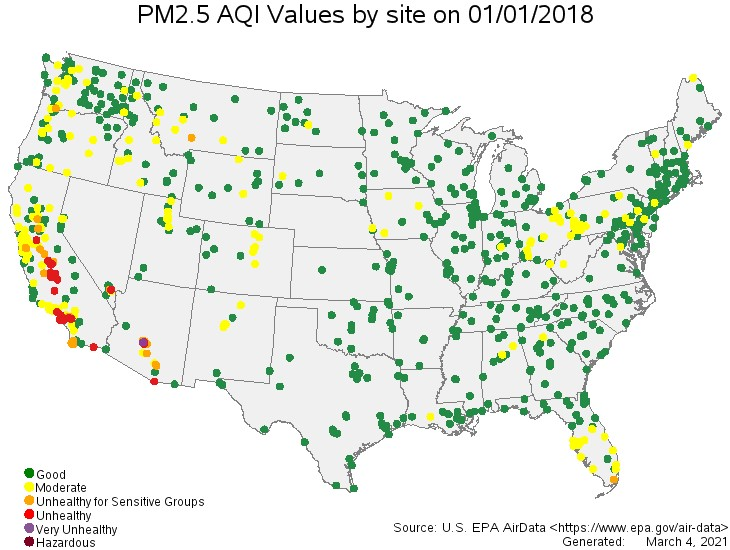
\includegraphics[scale=0.4]{images/AQ_US_2018.jpg}
    \caption{$PM_{2.5 }$ AQI Values}
\end{figure}

%% The next two lines define the bibliography style to be used, and
%% the bibliography file.
\bibliographystyle{ACM-Reference-Format}
\bibliography{references}

\end{document}
\endinput
